%================================================================
\section{Results}\label{sec:results}
% Present results and give a critical discussion of my work in 
% the context of other work. Relate the work to previous studies, 
% and make sure the results are reproducible. Include information 
% in figure captions such that they can give the reader enough to 
% understand the main gist of the report.
%================================================================

\subsection{Gradient descent}

We applied the gradient descent algorithm to data simulated from a third-degree polynomial without noise to assess convergence to the true parameters (APPENDIX). All parameters converged after approximately 800 iterations using plain gradient descent (figure \ref{fig:poly-converge}). Adding momentum to the gradient descent sped up convergence to around 4-fold (figure \ref{fig:poly-converge-momentum}), and using any optimizer had similar effects on convergence times (APPENDIX FIGS).

\begin{figure}
    \centering
    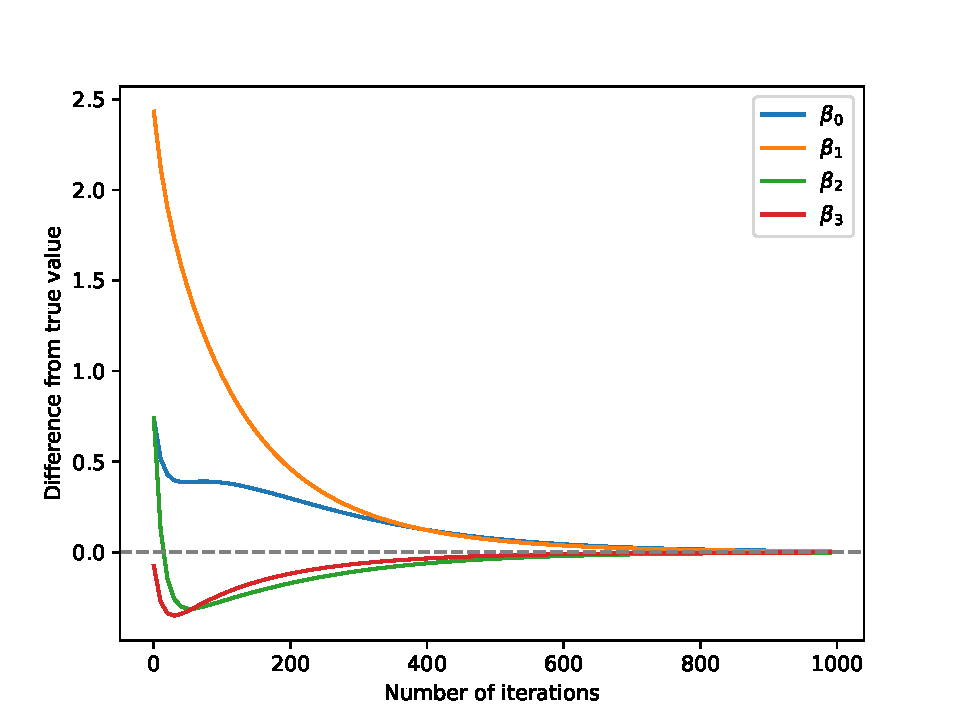
\includegraphics[width=0.99\linewidth]{examples/tests_even/figs/gradient-descent-polynomial-convergence.pdf}
    \caption{Gradient descent on data generated from a 4th degree polynomial without noise, using polynomial features up to the 4th degree. The stippled line represents 0 difference from the parameters used to generate the data.}
    \label{fig:poly-converge}
\end{figure}

\begin{figure}
    \centering
    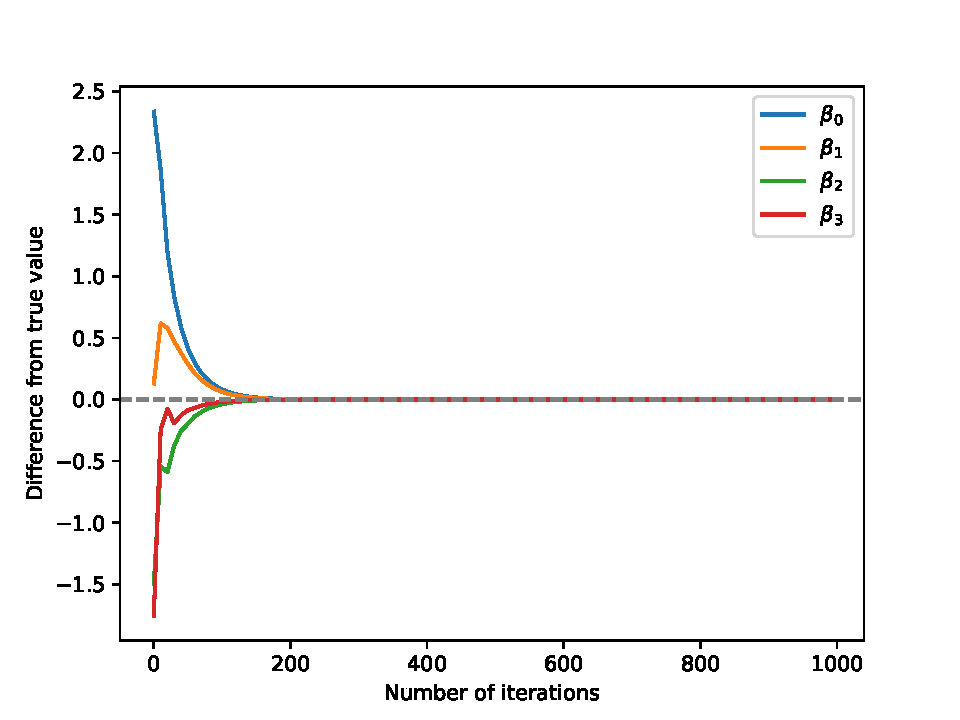
\includegraphics[width=0.99\linewidth]{examples/tests_even/figs/gradient-descent-momentum-polynomial-convergence.pdf}
    \caption{Gradient descent on the same data as in Figure \ref{fig:poly-converge}, but using momentum. The algorithm converged considerably faster than gradient descent without momentum.}
    \label{fig:poly-converge-momentum}
\end{figure}

The choice of learning rate affected the performance of the model regardless of optimizer. For data generated from the Franke function \cite{franke1979} with added noise, the different optimizers had different optimal learning rates, but in general a learning rate between $10^{-3}$ and $1$ gave the best results (figure \ref{fig:franke-learningrate}). For this particular data GD outperformed SGD (APPENDIX). Overall, ADAM consistently gave the lowest mean squared error on the test data over the largest range of learning rates. Because of this, we chose to emphasize ADAM over the other optimizers when analyzing the terrain data.   

\begin{figure}
    \centering
    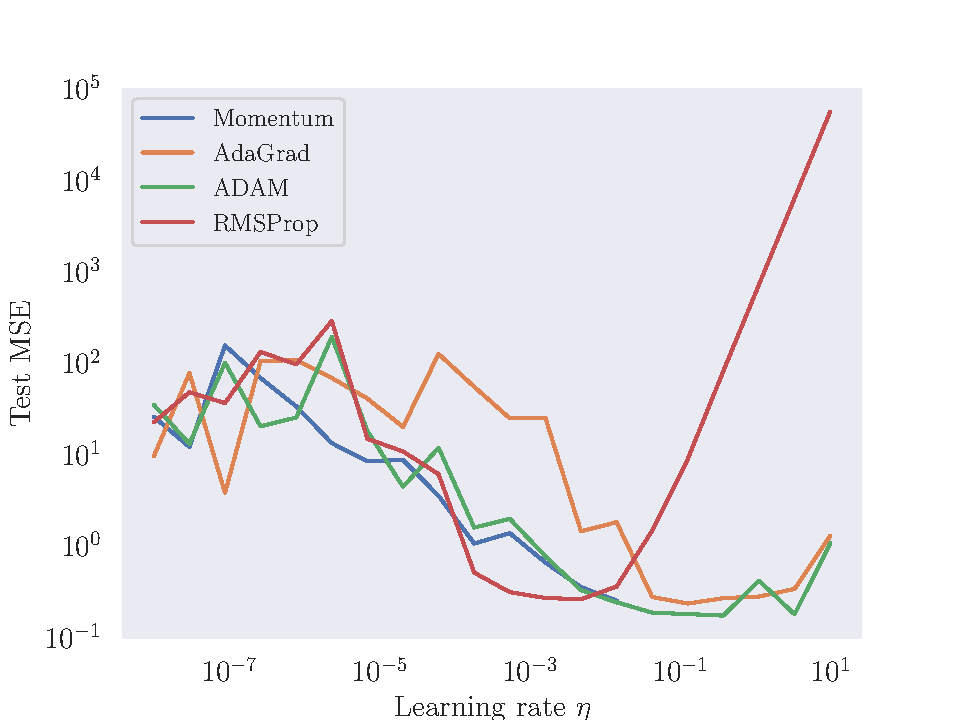
\includegraphics[width=0.99\linewidth]{examples/tests_even/figs/Franke-learningrates-optimizers.pdf}
    \caption{How learning rates affect the mean squared error in gradient descent with momentum or different optimizers. The data was generated from the Franke function, with added noise. For the momentum algorithm the gradient descent was not completed for learning rates above $10^{-2}$ due to exploding gradients.}
    \label{fig:franke-learningrate}
\end{figure}

- describe implementation\\
- Show all the different optimizers etc\\
- compare to regression from last project\\
- Based on this, we chose to keep this and this optimizer\\
- include figure of terrain, compare to ridge from last project and data\\



\subsection{Regression analysis with FFNN}

- compare to project 1\\
- discuss results compared to OLS/Ridge\\
- Optimal learning rates and parameters, lambda-learningrate grid-search\\
- discuss activation functions\\
- discuss initialization of learning rates\\


\subsection{Breast cancer data}
- A couple of sentences on choosing optimizer
- Classification and accuracy of binary classification\\
- Discuss the results and analyze the different parameters used (learning rate, lambda) and the effect of different activation functions\\
- Compare with similar code from Scikit-Learn etc.\\
- Compare with logistic regression\\



Future works: 
- Dropout rate to prevent overfitting
- 